\section{Aufgabe 1 -- Hindernisvermeidung (Jan)}

Damit ein mobiler Roboter eine Karte von einem Raum aufnehmen kann muss er sich natürlich durch den Raum bewegen können um alle Ecken zu erreichen. Dabei ist es unumgänglich eine Strategie zu implementieren mithilfe derer der Roboter durch den Raum fährt ohne mit Hindernissen und Wänden zu kollidieren.
Da der Laserscanner eine Reichweite von etwa 8 Metern hat muss der Raum nicht unbedingt systematisch abgefahren werden. Es reicht, wenn der Roboter alle Ecken des Raumes mit dem Laserscanner mindestens einmal aufnehmen kann. In Abbildung~\ref{fig:kartonRaumLabor} ist ein Testbereich zu sehen, der im Labor mithilfe von Pappkartons aufgebaut wurde. Der Roboter soll zum Beispiel in diesem Bereich eine Karte aufnehmen können.

\begin{figure}[H]
	\centering
	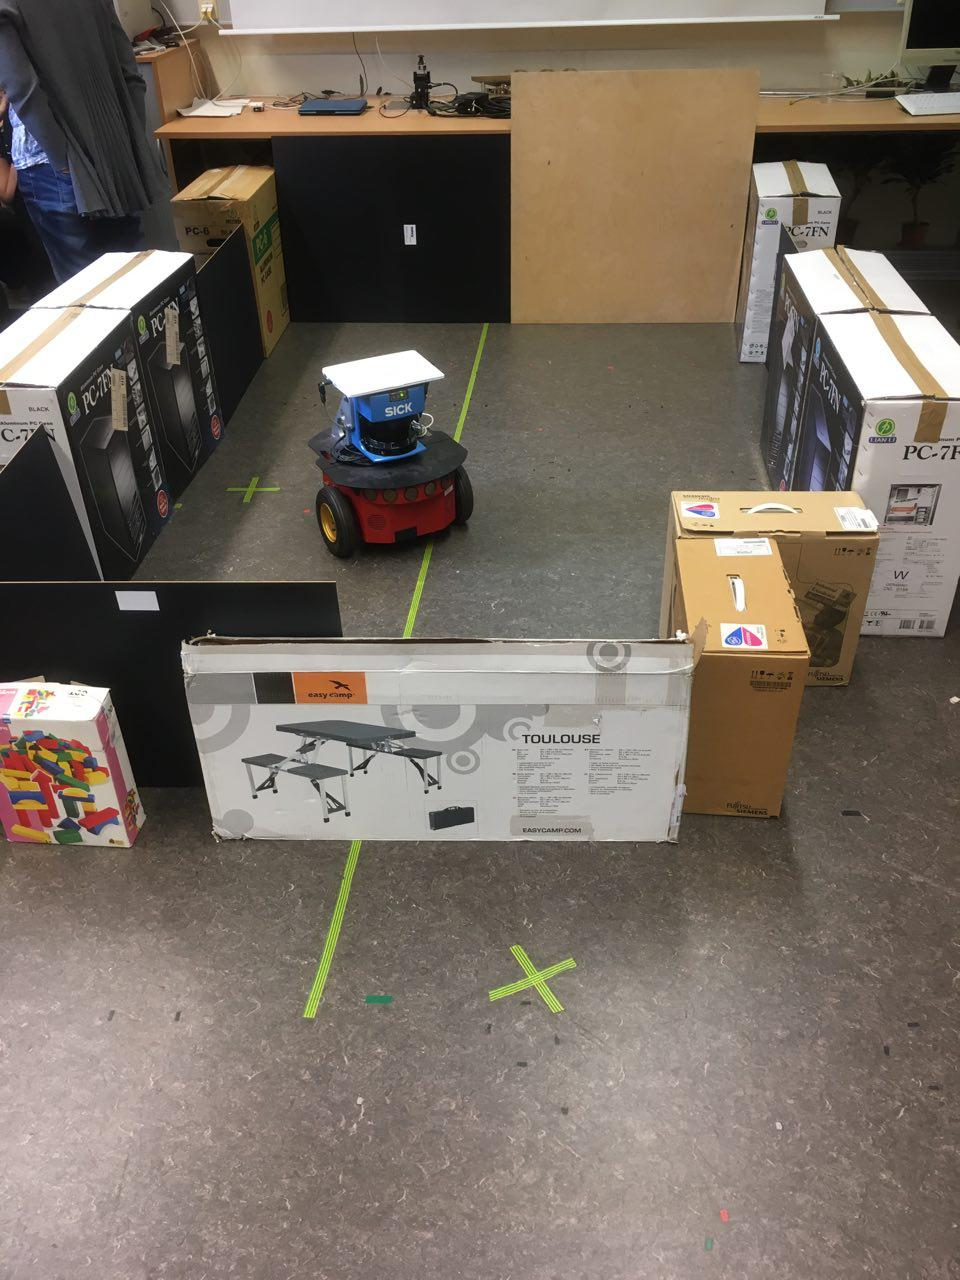
\includegraphics[width=10cm]{kartonRaumLabor}
	\caption{Der Roboter in einem mithilfe von Kartons errichteten Testbereich für das Aufnehmen einer Karte.}
	\label{fig:kartonRaumLabor}
\end{figure}

Die Strategie, die wir zuerst implementiert haben, war es leicht vom nächsten Hindernis weg zu lenken. Es wird der Scanpunkt mit dem minimalen Abstand bestimmt und wenn dieser eher auf der rechten Seite des Roboters liegt wird leicht nach links gesteuert, bzw. falls das nächste Hindernis sich eher links befindet, wird leicht rechts gesteuert. Wenn der minimale Abstand aber über einem Threshold von 1,2 Metern liegt, fährt der Roboter einfach weiter geradeaus.

Ein Problem mit diesem Ansatz trat auf, falls der Roboter in eine Sackgasse gefahren war und dann schräg vor einer der Ecken stand.
Dies haben wir zunächst versucht durch eine Sackgassenerkennung zu beheben, die auf ein lokales Maximum geradeaus vor dem Roboter prüft.
Leider hat dieser Lösungsansatz nicht so gut funktioniert und häufig wurde der Autostop des Roboters ausgelöst. Da wir ein weiteres Problem dieses Ansatzes mit Löchern in den Wänden (zwischen den Kartons) sahen, haben wir uns entschieden den Ansatz zu wechseln.

Der neue Ansatz soll nun zum Einen das Problem der Sackgassen lösen und zum Anderen auch mit Spalten zwischen den Wänden klarkommen. Dazu werden die Scanpunkte zunächst in 3 gleich große Bereiche aufgeteilt. Der erste Bereich sind die Punkte, die zur rechten Seite des Roboters liegen. Der zweite Bereich sind die Punkte, die geradeaus vor dem Roboter liegen und der dritte Bereich sind schließlich die Punkte, die links vom Roboter liegen. In jedem der Bereiche werden nun die Scanpunkte gezählt, die einen bestimmten Distanzthreshold unterschreiten. Zunächst haben wir den Threshold auf 1,2 Meter gesetzt, damit wir mit aktivem Autostop testen konnten.
Für die Anzahl Scanpunkte, ab dem ein Bereich als ''nah'' gilt wurde ein Threshold auf 5 Stück festgelegt. Dies verhindert, dass durch Ausreißer eine Hindernisvermeidung angestoßen wird und schlägt trotzdem direkt an, falls ein echtes Hindernis im Weg auftauchen sollte.
Falls sich im vorderen Bereich nun weniger Scanpunkte befinden als dieser Threshold, wird einfach weiter der alte Ansatz verfolgt. Wenn sich allerdings im vorderen Bereich ein Hindernis befindet verhält sich der Roboter anders. Zunächst vergleicht er die Anzahl Scanpunkte auf der linken und der rechten Seite deren Distanz unter dem Threshold ist. Falls links weniger Punkte als rechts sind fährt er eine scharfe links Kurve, falls rechts weniger Punkte sind eine scharfe rechts Kurve. Falls aber auf beiden Seiten ungefähr gleich viele Punkte sind und die Punkteanzahl den Threshold von 5 Punkten überschreitet geht er von einer Sackgasse aus und versucht sich umzudrehen indem er auf der Stelle dreht. Falls auf beiden Seiten ungefähr gleich viel Platz scheint fährt er einfach eine scharfe rechts Kurve.

Dieser Ansatz funktioniert ziemlich gut und wir konnten den Autostop deaktivieren um zu testen wie weit wir den Distanzthreshold verringern können. Letztendlich haben wir den Threshold auf 0,7 Meter heruntergesetzt. Der Roboter vermeidet Hindernisse nun sehr zuverlässig ohne aber Ecken eines Raumes komplett auszulassen. Er schafft es sogar selbstständig durch die Labortür auf den Flur.